\section{Classical attack vectors} \label{classical-attack-vectors}

Any cryptosystem is vulnerable to attacks and this piece wouldn't exist if they weren't. Attacks come in many shapes and forms, some computational, others not. We begin by discussing classical attack vectors, which refers to attacks using only classical resources, which may or may not be computational in nature.

\subsection{Backdoors} \label{backdoors}

By far the most powerful classical attack vectors are \emph{backdoors}, whereby cryptography is bypassed altogether, providing direct access to plaintext data. This could be achieved in a number of ways:
\begin{itemize}
	\item Malware could be installed onto clients' devices that directly accesses plaintext data streams and sends them to the attacker. Malware could find its way onto devices via malicious code (e.g that link you pressed on that strange SMS you received), or directly installed, as has often been the case by human intelligence (HUMINT) agencies penetrating physical security measures. Malware attacks can indeed offer far greater utility than simply intercepting data, and can be used to control client devices for other purposes, including sending fraudulent data. Perhaps the most famous example of malware being used by a nation-state was Israel's installation of the Stuxnet malware onto the computers controlling Iran's nuclear centrifuges, destroying a significant number of them, setting back Iran's nuclear program by years according to some estimates.
	\item Targets are tricked into using encryption algorithms that have vulnerabilities known to the attacker but no one else. It has often been speculated that the NSA manipulated standardised encryption algorithms to this end, although this has not been firmly established.
	\item Governments use their legislative power to force computer hardware and software manufacturers to hard code backdoors into devices granting government agencies direct access to client-side data. This is effectively a malware attack by decree, but one only available to governments with jurisdictional power over the companies manufacturing devices. World governments have for a long time become increasingly hostile to the availability of strong end-to-end encryption on consumer-grade devices, with a long history of lobbying the tech sector to introduce backdoors, lamenting the missed opportunities for law enforcement and intelligence agencies. Although not admitted, it should be taken for granted that such backdoors exist in major commercial operating systems and hardware. For example, as described in \href{https://peterrohde.org/apples-child-protection-software-is-not-about-child-safety-its-a-government-backdoor/}{this article}, Apple's child safety framework by the nature of its design is a clear client-side, government backdoor, and by virtue of the people implementing it clearly isn't something that's intended with child safety as the leading priority (although using the justification `child safety' is the leading way to shut down any political opposition to it and inhibit transparency into what data is collected).
\end{itemize}

Backdoors in any incarnation can be regarded as \emph{post-quantum attack vectors} --- if you have direct access to client-side data it simply doesn't matter how strong your encryption with other parties is. Bearing in mind that any system is only as secure as any single point of failure --- of which backdoors are one --- this is a type of attack that transcends eras and technologies, and must always be a priority in secure systems.

One of the strongest protections against backdoors is to rely on open-source software (both for operating systems and applications), allowing anyone to independently audit the code with complete transparency. This is one of the leading reasons why the security of open-source messaging apps such as Signal is considered more robust and reliable than proprietary, closed-source apps which lack this transparency and the ability for independent auditing.

\subsection{Side-channel attacks} \label{side-channel-attacks}

A side-channel attack is one that exploits differences between the theory and implementation of a cryptosystem. Theory almost always makes highly idealised assumptions which are difficult to perfectly reflect in practise. Should these differences provide correlations that can be exploited to gain secret information, it provides avenues for attack. Side-channel attacks exist both for classical and quantum cryptography, however quantum systems are arguably more vulnerable due to the greater difficulties in making experiment perfectly match theory and that classical systems are far better studied.

\subsection{Hammer attacks} \label{hammer-attacks}

One of the most successful classical attack vectors, effectively a form of backdoor, is the \emph{hammer attack}, whereby the adversary kidnaps a party possessing a private key, holds a hammer above their head and says ``give me the key''. Despite finding widespread historical use in the field of espionage, this attack vector is considered a high-risk one, typically only employed in very extreme scenarios, for very high-value information. They also suffer the disadvantage that they are not opaque, typically resulting in the target becoming aware that they have been compromised.

\subsection{Cryptanalysis} \label{cryptanalysis}

Cryptanalysis is the field of using computational and mathematical methods to break ciphers based on computational security assumptions.

\subsubsection{Brute-force attacks} \label{brute-force-attacks}

A brute-force attack is the most primitive and inefficient means by which to crack a code. The idea very trivially is to exhaustively search the key space and decrypt the ciphertext using each key to see if something sensible comes out. This type of attack has two main problems, which is why it is not typically viable to employ:
\begin{itemize}
	\item For an $n$-bit key there are $2^n$ possible keys, which is a highly unfavourable exponential in $n$. Searching through $2^{256}$ keys isn't viable on any kind of computer. Even a quantum computer employing Grover's algorithm (Sec.~\ref{grovers-algorithm}) will only reduce this by a quadratic factor, yielding $2^{n/2}$, which is still an astronomical exponential, just reducing the effective key-length by a factor of a half, which can easily be compensated for by doubling key-lengths to begin with.
	\item Since this is a computational attack it only applies to cryptosystems based on \emph{computational security}. Ones based on \emph{information theoretic security}, like the one-time-pad and various other quantum encryption techniques, make them immune to computational attacks.
\end{itemize}

There have been demonstrations of brute-force attacks breaking DES (Digital Encryption Standard) encryption, a now outdated standard using a 64-bit block and key size. However, modern symmetric ciphers have transitioned to 128- and 256-bit block/key lengths, ruling out any future possibility of vulnerability to brute-force attacks (including quantum attacks for the larger key sizes).

\subsubsection{Known-plaintext attacks} \label{known-plaintext-attacks}

A known-plaintext attack is a cryptanalytic attack whereby the eavesdropper happens to know both the plaintext and ciphertext of a given message. Then based on some advanced mathematical analysis, dependent on the type of encryption, the key can be inferred, or at least partially. With the one-time-pad, for example, this is trivial --- we simply XOR the plaintext and ciphertext to directly determine the key. However, in this example knowing the key isn't especially useful since by definition it is never reused.

The most famous successful case of this type of attack was that of Alan Turing's efforts to decrypt the German Enigma machine during the Second World War. Based upon various pieces of known information in decrypted messages obtained via other intelligence means, Turing's team was able to reverse engineer keys. Turing's success in cracking the Enigma machine has widely been regarded as a pivotal factor in Germany's defeat.

Modern ciphers are designed and believed to be robust against this type of attack.

\subsubsection{Differential
cryptanalysis} \label{differential-cryptanalysis}

Differential cryptanalysis is the study of how differences in inputs to a cipher propagate through and translate to differences in the outputs. Such techniques could be applicable in a scenario of known plaintexts for slightly different inputs, from which the propagation of the difference between those plaintexts through the cipher is examined to attempt to extract key bits.

\subsection{Man-in-the-middle attacks} \label{man-in-the-middle-attacks}

There is one particularly nefarious attack, known as the \emph{man-in-the-middle} or \emph{intercept-resend} attack, which is notoriously hard to eliminate. As the name suggests, here an eavesdropper (Eve) sits in between two parties, fooling (aka `spoofing') both into thinking she is the other, intercepting all exchanged public keys and retransmitting new ones (see Figs.~\ref{fig:MIM_1} and \ref{fig:MIM_2}). She then has the absolute ability to intercept and decrypt all communications.

\begin{figure}[!htb]
	\centering
	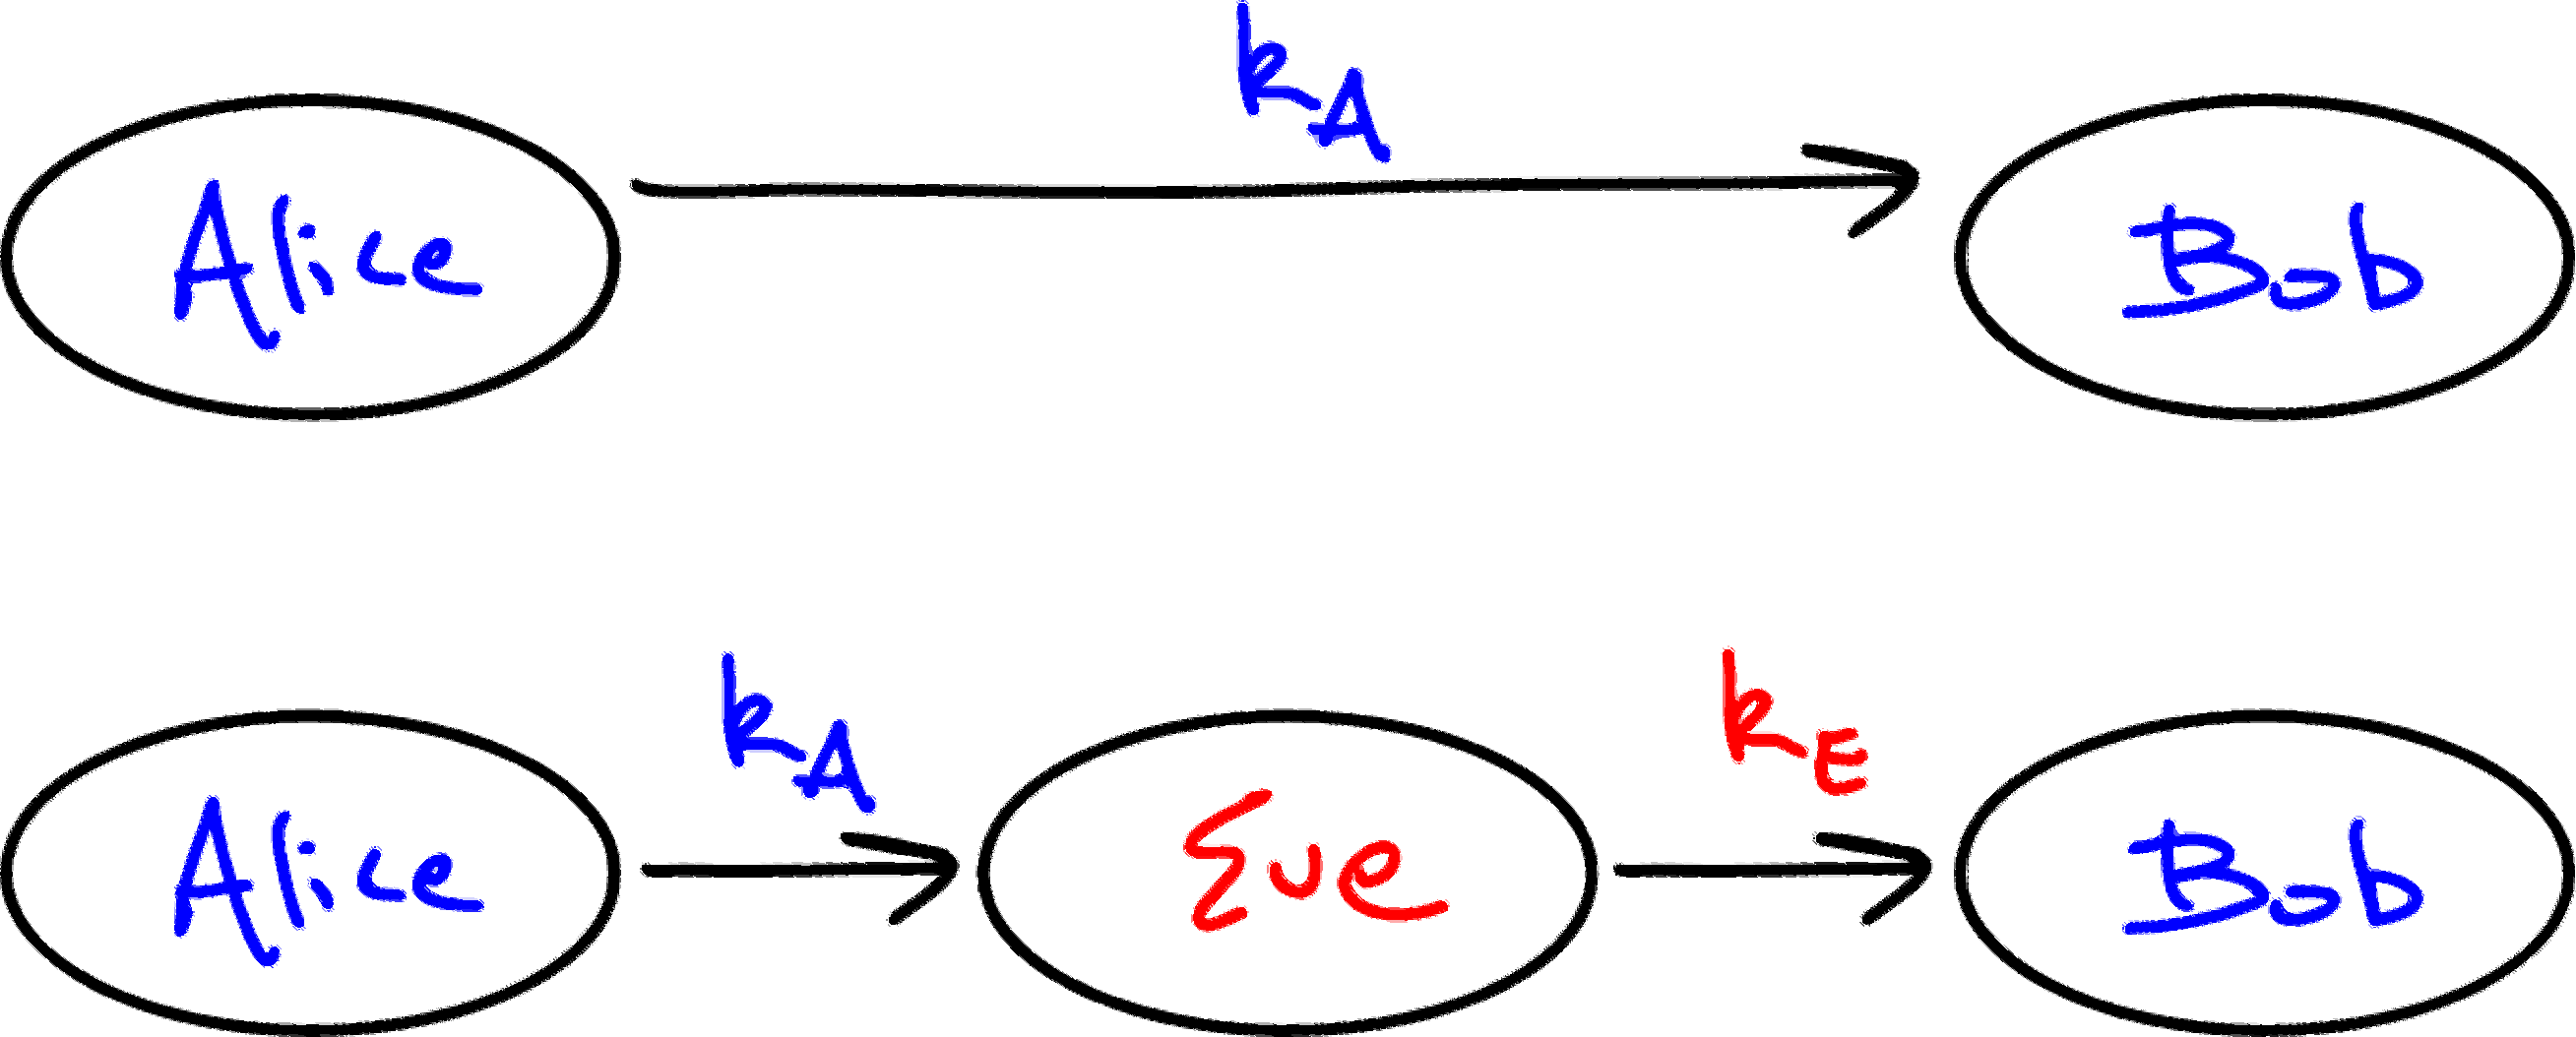
\includegraphics[width=\columnwidth]{figures/Intercept_resend_1}
	\caption{One-way intercept resend-attack. The eveasdropper Eve intercepts Alice's key, retransmitting her own to Bob, spoofing Bob into thinking she is Alice.} \label{fig:MIM_1}
\end{figure}

\begin{figure}[!htb]
	\centering
	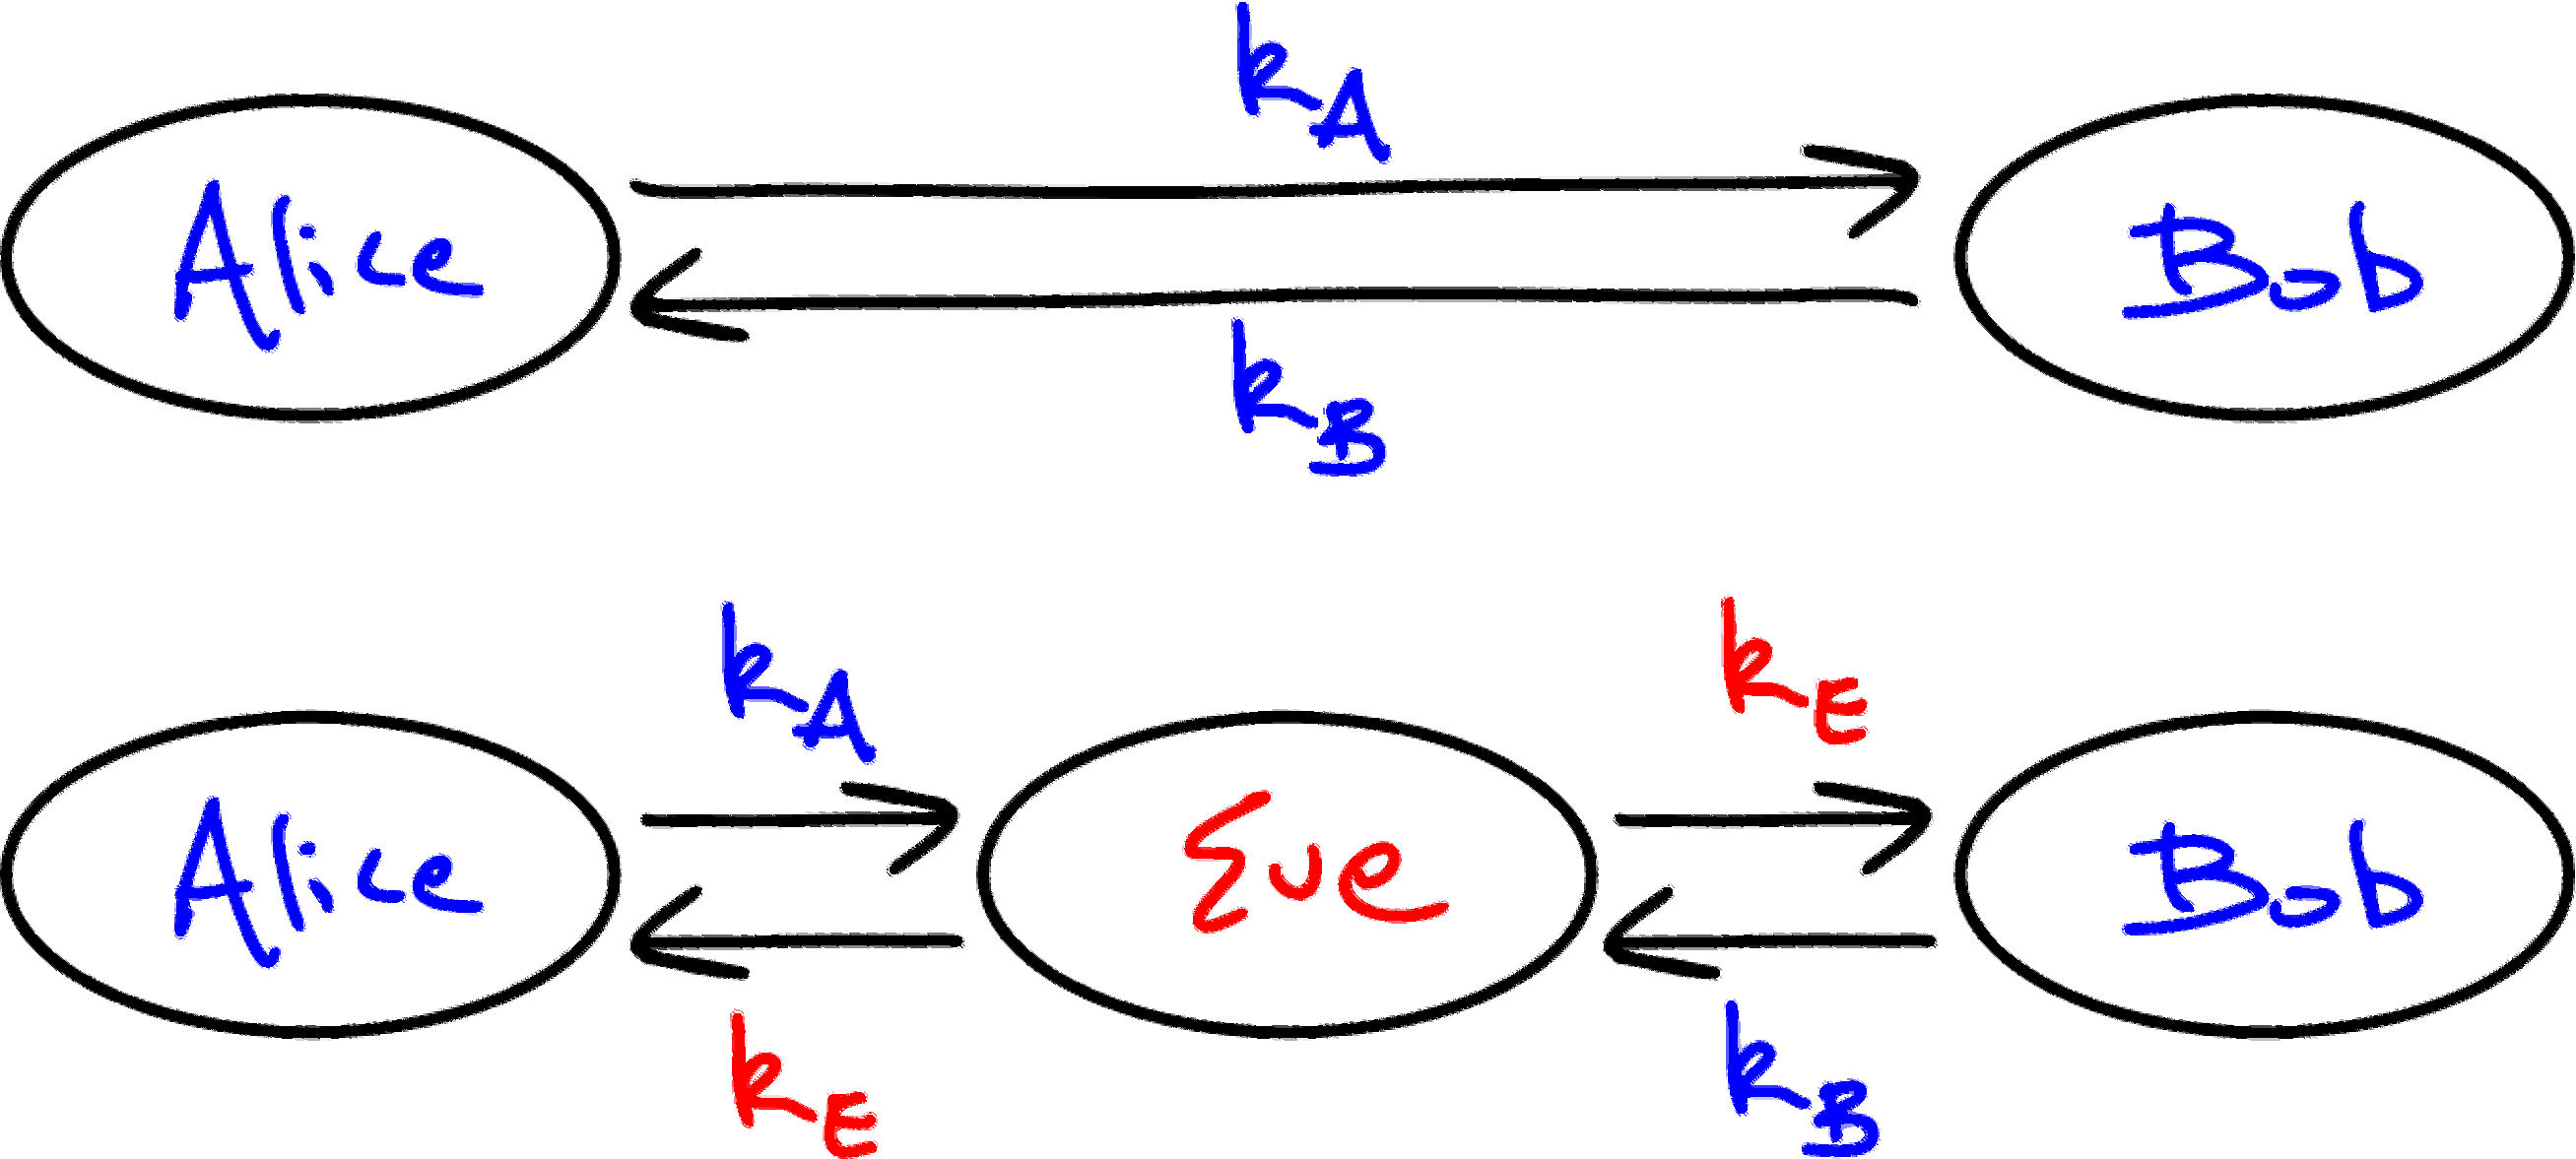
\includegraphics[width=\columnwidth]{figures/Intercept_resend_2}
	\caption{A two-way intercept-resend attack operates the same way as a one-way intercept-resend attack, except in both directions simultaneously, spoofing both Alice and Bob into thinking that she is the other.} \label{fig:MIM_2}
\end{figure}

The only way to truly eliminate man-in-the-middle attacks is for the two parties to have some way of identifying the other. This could be in the form of confidently knowing their public key or having a shared secret key for authentication. In either case, this requires having some trusted means of establishing the authenticity of the authenticating key. For two parties who have never met this becomes logistically tricky, especially in a globalised environment.

\subsubsection{Signature fingerprints}

The Signal messaging app attempts to mitigate this issue by periodically asking users to compare \emph{safety numbers} (see Fig.~\ref{fig:safety_num}), which are just a fingerprint of both parties' public keys,
\begin{align}
	\texttt{fingerprint}_{A,B} = \texttt{hash}(\texttt{hash}(\mathrm{pub}_A)\oplus\texttt{hash}(\mathrm{pub}_B)).
\end{align}

If the safety numbers match it implies they are both using the correct public keys, thereby ruling out a man-in-the-middle. However for this comparison to be meaningful it must take place via an alternate channel that is not likely to be simultaneously compromised by the same man-in-the-middle. For example, users could meet in person to compare numbers (or simply scan the associated QR codes). With slightly less security they could share it via a different digital channel, or by a voice/video call which is hard for a man-in-the-middle to mimic.

\begin{figure}[!htb]
	\centering
	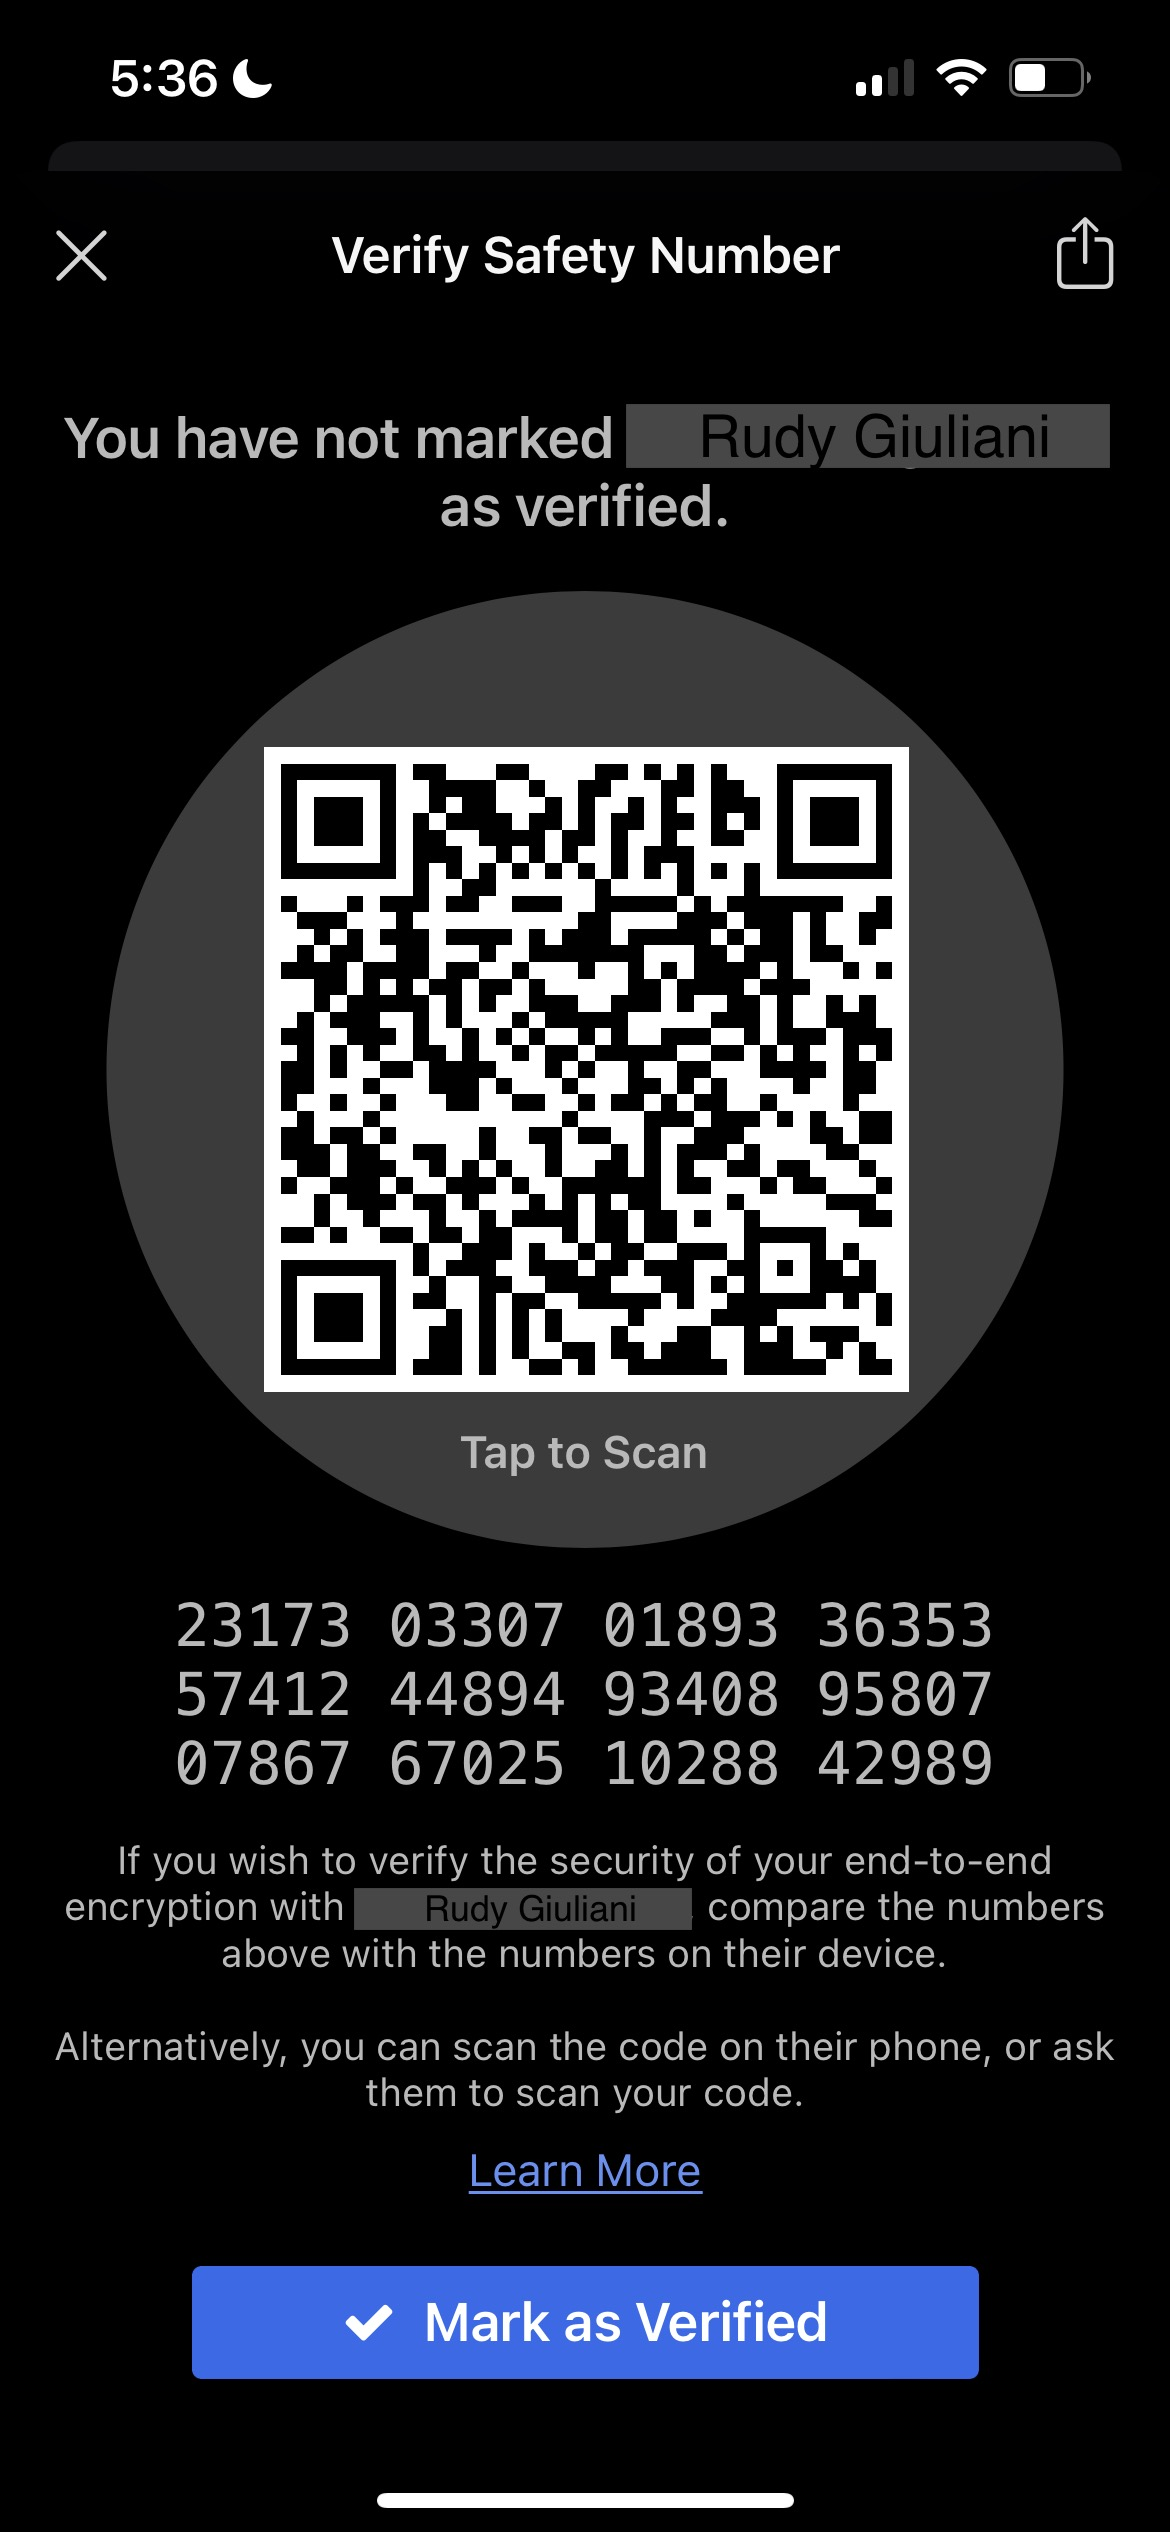
\includegraphics[width=0.8\columnwidth]{figures/Safety_number.jpeg}
	\caption{Safety numbers in the Signal messaging app provide a fingerprint of the users' public keys. When compared via a trusted channel, which needn't be secret, this provides confirmation that the two parties are using one another's public keys, thereby ruling out a man-in-the-middle attack.} \label{fig:safety_num}
\end{figure}

\subsubsection{Certificate authorities} \label{certificate-authorities}

While the previous approach of manually comparing fingerprints might be practical for a messaging app, it isn't viable for more general communications systems, especially ones that communicate with parties they have not previously interacted with, i.e much of the internet.

If we're to rely on public-key cryptography, whether for encryption or digital signatures, how can we ensure the other party actually is who we think it is and isn't being spoofed? How do we know the published public-key we obtained is actually theirs? There are two approaches here:
\begin{enumerate}
\item The public-key is securely shared, requiring some form of secret communication. This somewhat bypasses the whole point of public-key cryptography, which is to avoid the need for secret communication, in which case we'd might as well use private-key cryptography, which is far more robust against quantum attack vectors.
\item We rely on trusted third parties to act as guarantors to vouch for the integrity of the public-keys of others, so-called \emph{certificate authorities}.
\end{enumerate}
%The answer is that somewhere along the line we need to rely on trusted third parties who act as guarantors of the validity of the public keys of others. These trusted third parties are often called \emph{certificate authorities}, who we outsource the hard work of establishing the authenticity of others to.

The latter is the most practical and commonplace method to achieve this (see Fig.~\ref{fig:certificate}). However, since this model relies on trust, it introduces a point of failure -- how do we ensure that the certificate authority itself isn't being spoofed and hasn't been compromised? At some point along the line we are going to have to rely upon the former approach. That is, no matter who we rely on for obtaining the public-keys of others, at some stage we need secure communication to have a trusted public-key for at least \emph{someone}.

For this reason, when you purchase a new computer or mobile phone the pre-installed operating system will have the public-keys of some trusted agencies, such as Apple, Google and/or some other certificate authorities, hard-coded to address this problem. This means spoofing these trusted agencies would require compromising physical devices prior to being sold, a challenging endeavour.

\begin{figure}[!htb]
	\centering
	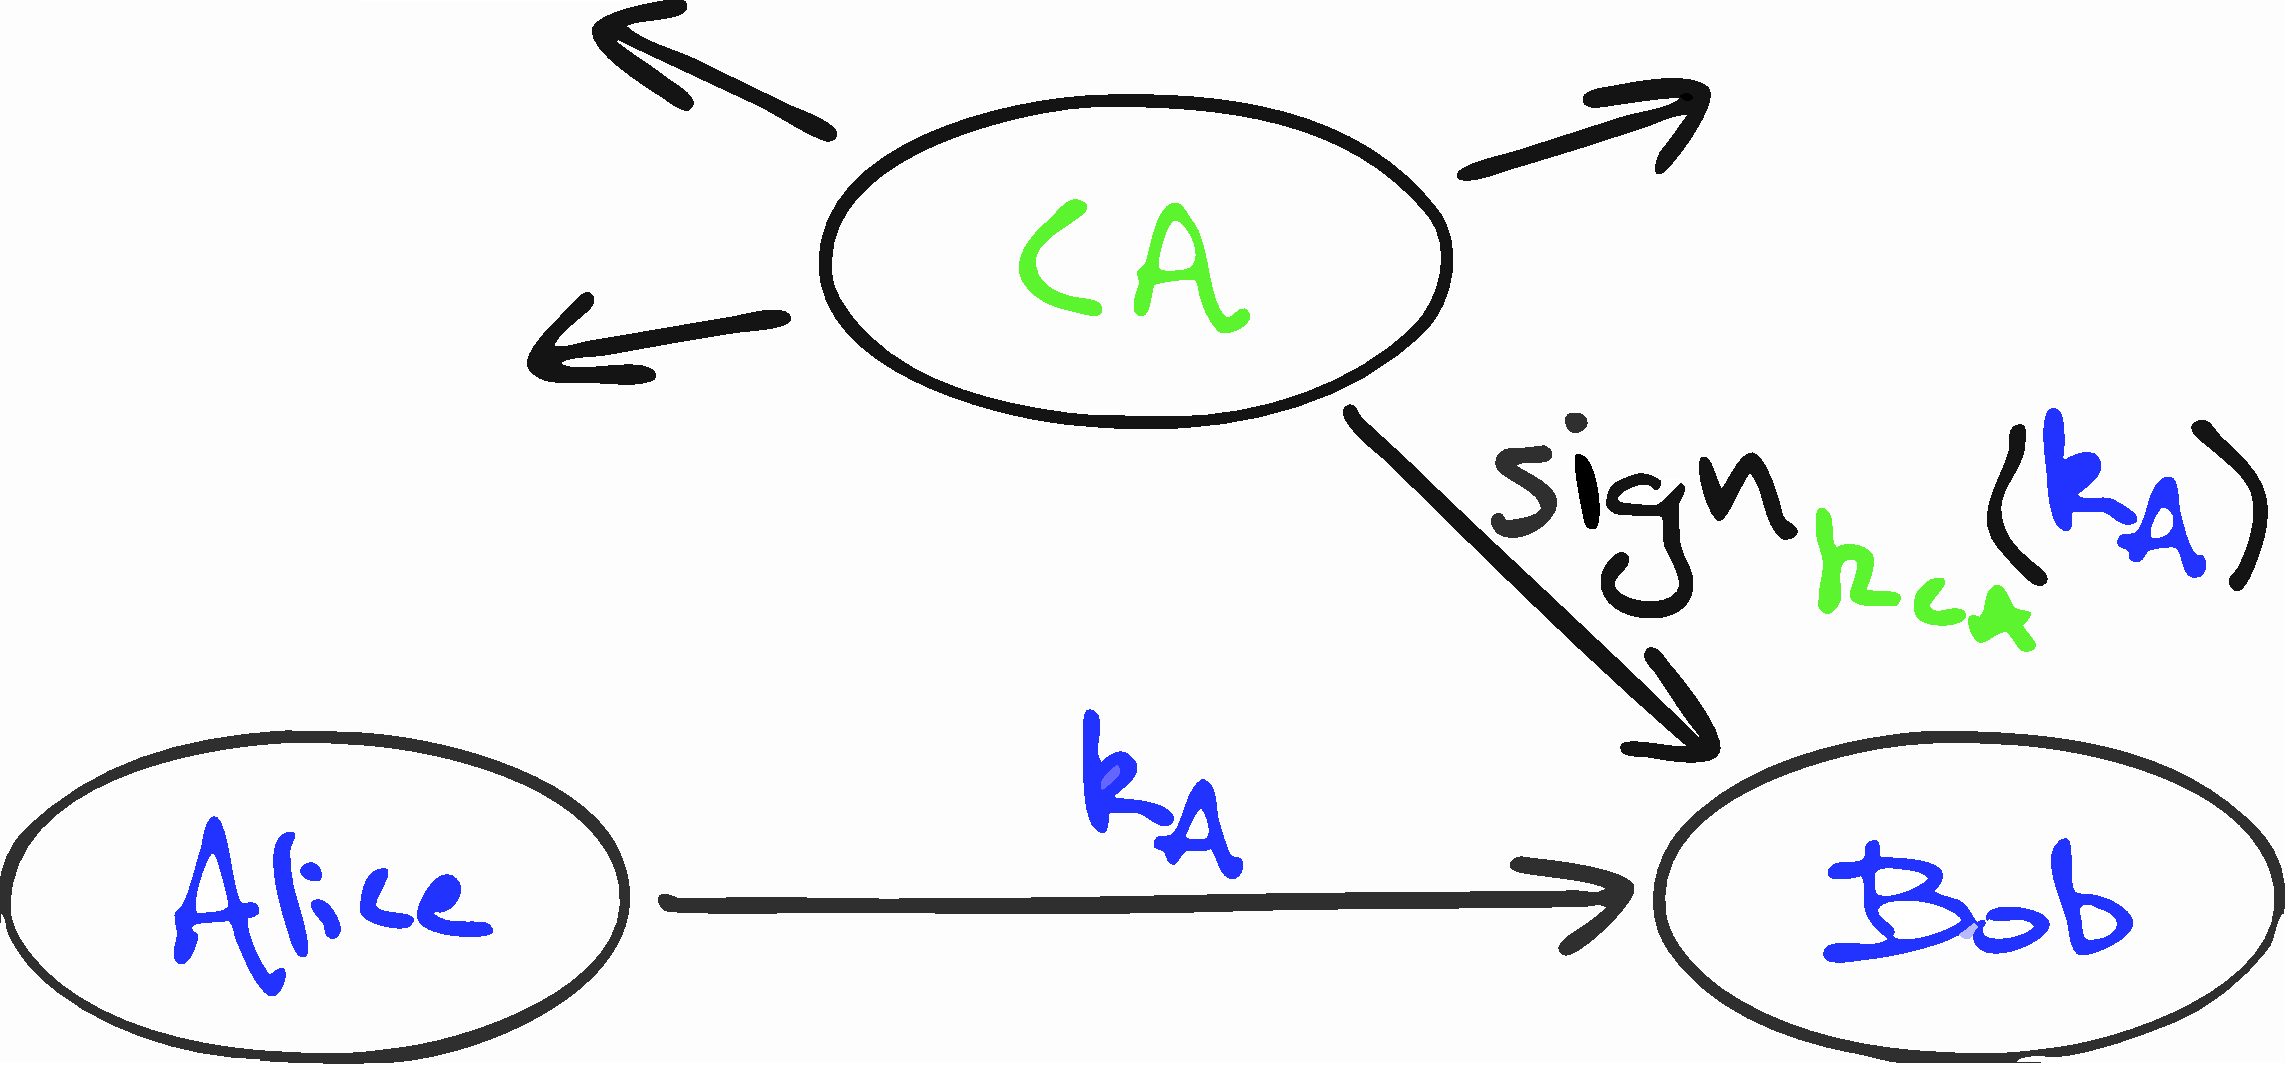
\includegraphics[width=\columnwidth]{figures/Certificate_authority}
	\caption{A certificate authority is a central, trusted agency who signs off on the public keys of other parties, confirming their authenticity. This helps reduce the risk of man-in-the-middle attacks inserting themselves between unknown parties and spoofing them. Here, Alice communicates her public key, $k_A$, to Bob to allow him to securely communicate with her. Bob can't be sure that an eavesdropper Eve isn't inserting herself in between and spoofing Alice, so he queries the trusted certificate authority (CA) who signs Alice's signature to vouch for its integrity, $\mathtt{sign}_{k_{CA}}(k_A)$. Now if Eve is to successfully spoof Alice, she must also compromise or spoof the certificate authority.} \label{fig:certificate}
\end{figure}